\chapter{蒙特卡洛与时序差分学习}

\intro{模型无关的强化学习——不需要知道环境的转移概率和奖励函数，仅通过与环境的交互经验来学习最优策略。}

\section{引言：从模型已知到模型未知}

在前三章中，我们建立了马尔可夫决策过程（MDP）的理论框架，并讨论了动态规划方法。动态规划（如策略迭代和值迭代）的核心前提是我们必须知道环境的完整模型——即状态转移概率 $\trans(s'|s,a)$ 和奖励函数 $\reward(s,a)$。然而，在大多数实际应用中，这些模型信息是未知的。我们不可能提前知道一个机器人从某个关节角度移动到另一个角度的精确概率分布，也无法预知金融市场对某个交易行为的精确反应。

本章和下一章将重点讨论\textbf{模型无关的强化学习}（Model-Free RL），即智能体无需了解环境的内部动态，仅通过与环境的实际交互来学习。模型无关方法可以分为两大类：

\begin{enumerate}
    \item \textbf{蒙特卡洛方法}（Monte Carlo, MC）：通过完整的轨迹（episode）来估计值函数，适用于回合制（episodic）任务。
    \item \textbf{时序差分方法}（Temporal Difference, TD）：通过单步或少量步骤的转移来更新值函数，既可用于回合制任务，也可用于连续任务。
\end{enumerate}

这两种方法的巧妙结合与扩展构成了现代深度强化学习的理论基石。

\begin{mydefinition}{模型无关学习（Model-Free Learning）}
模型无关学习是指智能体在不拥有环境模型 $\trans$ 和 $\reward$ 的情况下，仅通过与环境交互获得的经验数据 $(S_t, A_t, R_{t+1}, S_{t+1})$ 来学习值函数或策略的方法。
\end{mydefinition}

\begin{tikzpicture}[auto, node distance=2.5cm, thick]
    \node[draw, rounded corners, fill=blue!10, text width=3cm, align=center] (dp) {动态规划\\(DP)\\需要完整模型};
    \node[draw, rounded corners, fill=red!10, text width=3cm, align=center, right=of dp, xshift=2cm] (mc) {蒙特卡洛\\(MC)\\仅需经验, 无模型};
    \node[draw, rounded corners, fill=green!10, text width=3cm, align=center, right=of mc, xshift=2cm] (td) {时序差分\\(TD)\\仅需经验, 无模型};
    
    \draw[->, >= stealth, line width=0.8pt] (dp) -- node[above, text width=2cm, align=center, font=\footnotesize] {增加模型\\依赖性} (mc);
    \draw[->, >= stealth, line width=0.8pt] (mc) -- node[above, text width=2cm, align=center, font=\footnotesize] {减少方差\\增加偏差} (td);
\end{tikzpicture}

\section{蒙特卡洛方法}

\subsection{从经验中学习}

蒙特卡洛方法基于一个朴素而强大的思想：通过对随机样本的平均来估计未知量。在强化学习中，"样本"就是一条完整的经验轨迹（episode），"未知量"是状态值函数 $v_{\pi}(s)$ 或动作值函数 $q_{\pi}(s,a)$。

\begin{mydefinition}{蒙特卡洛方法（Monte Carlo Method）}
给定策略 $\pi$，蒙特卡洛方法通过从该策略出发的完整回合中观察到的实际累计回报（return）来估计值函数。具体而言：
$$v_{\pi}(s) \doteq \E_{\pi}[G_t \mid S_t = s] \approx \frac{1}{N}\sum_{i=1}^{N} G_t^{(i)}$$
其中 $G_t^{(i)}$ 是第 $i$ 条轨迹中从状态 $s$ 首次出现时的实际回报。
\end{mydefinition}

考虑一个简单的网格世界示例来理解 MC 的采样过程：

\begin{example}
在一个 $3\times 3$ 的网格世界中，智能体从左上角出发，每次可以选择上、下、左、右四个动作（确定性执行）。到达右下角的目标位置获得 $+1$ 的奖励并终止。其他位置奖励为 $0$。策略为均匀随机策略 $\pi(a|s) = 1/4$。

图\ref{fig:mc-sampling} 展示了两条从该策略出发的采样轨迹，以及如何利用它们估计值函数。
\end{example}

\begin{figure}[H]
\centering
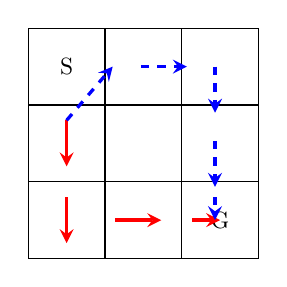
\begin{tikzpicture}[scale=0.65, every node/.style={scale=0.85}]
    % Grid world
    \draw[step=1.5, black, thin] (0,0) grid (4.5,4.5);
    
    % Labels
    \node at (0.75,3.75) {S};
    \node at (3.75,0.75) {G};
    
    % Trajectory 1 arrows (drawn manually)
    \draw[->, >= stealth, red, line width=1.2pt] (0.75,2.7) -- (0.75,1.8);
    \draw[->, >= stealth, red, line width=1.2pt] (0.75,1.2) -- (0.75,0.3);
    \draw[->, >= stealth, red, line width=1.2pt] (1.7,0.75) -- (2.6,0.75);
    \draw[->, >= stealth, red, line width=1.2pt] (3.2,0.75) -- (3.75,0.75);
    
    % Trajectory 2 arrows
    \draw[->, >= stealth, blue, line width=1.2pt, dashed] (0.75,2.7) -- (1.65,3.75);
    \draw[->, >= stealth, blue, line width=1.2pt, dashed] (2.2,3.75) -- (3.1,3.75);
    \draw[->, >= stealth, blue, line width=1.2pt, dashed] (3.65,3.75) -- (3.65,2.85);
    \draw[->, >= stealth, blue, line width=1.2pt, dashed] (3.65,2.3) -- (3.65,1.4);
    \draw[->, >= stealth, blue, line width=1.2pt, dashed] (3.65,1.2) -- (3.65,0.75);
\end{tikzpicture}
\caption{MC 采样示意图：红色实线为轨迹1（右-下-右-右），蓝色虚线为轨迹2（右-右-下-下-下）。两条轨迹的回报分别用于更新所访问状态的值估计。}
\label{fig:mc-sampling}
\end{figure}

\subsection{First-Visit MC 与 Every-Visit MC}

在一条回合中，同一个状态可能被访问多次。根据计算状态值的方式不同，蒙特卡洛方法分为两种变体。

\begin{mydefinition}{First-Visit MC 与 Every-Visit MC}
\begin{itemize}
    \item \textbf{First-Visit MC}：对于每个状态 $s$，仅使用该状态在回合中\textbf{第一次出现}时的回报 $G_t$ 来更新 $V(s)$ 的估计。这意味着每个回合中每个状态最多贡献一个样本。
    \item \textbf{Every-Visit MC}：对于每个状态 $s$，使用该状态在回合中\textbf{每次出现}时的回报 $G_t$ 来更新 $V(s)$ 的估计。这意味着每个状态在同一个回合中可能贡献多个样本。
\end{itemize}
\end{mydefinition}

两种方法的具体差异如下：

\begin{myformula}
\textbf{First-Visit MC 策略评估}
\end{myformula}

\begin{myalgorithm}{First-Visit MC 策略评估}
\textbf{输入：} 待评估的策略 $\pi$

\textbf{初始化：}
\quad 对所有 $s \in \states$，任意初始化 $V(s)$
\quad 对所有 $s \in \states$，初始化一个空列表 $\text{Returns}(s)$

\textbf{循环}（对每个回合）：
\quad 使用策略 $\pi$ 生成一个完整的回合：$S_0, A_0, R_1, S_1, A_1, R_2, \ldots, S_{T-1}, A_{T-1}, R_T$
\quad $G \leftarrow 0$
\quad \textbf{循环} $t = T-1, T-2, \ldots, 0$：
\quad \quad $G \leftarrow \gamma G + R_{t+1}$
\quad \quad \textbf{如果} $S_t$ 在 $S_0, S_1, \ldots, S_{t-1}$ 中未出现过：
\quad \quad \quad 将 $G$ 添加到 $\text{Returns}(S_t)$
\quad \quad \quad $V(S_t) \leftarrow \text{average}(\text{Returns}(S_t))$
\end{myalgorithm}

\begin{remark}
两种方法在理论上都是无偏的（unbiased），但 Every-Visit MC 因为同一回合内的样本存在相关性，其方差通常比 First-Visit MC 大。随着回合数量趋于无穷大，两种方法都依概率收敛到真实值 $v_{\pi}(s)$。
\end{remark}

\subsection{MC 策略评估的收敛性}

蒙特卡洛方法对状态值的估计是\textbf{无偏的}。对于 First-Visit MC，我们有：
$$\E[V(s)] = v_{\pi}(s)$$

这是因为每次访问状态 $s$ 的回报 $G_t$ 的期望正是 $v_{\pi}(s)$，而样本均值是总体均值的无偏估计量。

但是，MC 估计器的一个显著缺点是\textbf{高方差}。回报 $G_t$ 的方差来自两个方面：
\begin{enumerate}
    \item 环境本身的内在随机性（随机转移和随机奖励）
    \item 策略的随机性（如 $\varepsilon$-贪心策略中的随机动作选择）
\end{enumerate}

较长的回合通常会积累更多的随机性，导致回报方差更大。因此，MC 方法在处理长轨迹任务时效率较低。

\subsection{MC 估计动作值函数 $Q^{\pi}$}

在没有环境模型的情况下，仅知道状态值 $V(s)$ 是不够的。为了进行策略改进，我们需要知道动作值函数 $Q(s,a)$，因为策略改进需要比较不同动作的值：
$$\pi'(s) = \arg\max_a Q^{\pi}(s,a)$$

MC 方法以类似的方式估计 $Q(s,a)$：对每个状态-动作对 $(s,a)$，记录从该对出发所获得的实际回报，然后取平均值。

\begin{mydefinition}{MC 对 Q 值的估计}
$$Q(s,a) \approx \frac{1}{N(s,a)}\sum_{i=1}^{N(s,a)} G_{t}^{(i)}$$
其中 $N(s,a)$ 是状态-动作对 $(s,a)$ 被访问的次数，$G_{t}^{(i)}$ 是从该对被访问时开始的第 $i$ 次实际回报。
\end{mydefinition}

然而，当策略是确定性的（deterministic）时，某些动作可能从未被选择过，导致相应的 $Q(s,a)$ 无法被估计。这就引出了探索-利用（exploration-exploitation）的核心问题。

\subsection{探索与利用：Exploring Starts}

\begin{mydefinition}{探索-利用权衡（Exploration-Exploitation Trade-off）}
\begin{itemize}
    \item \textbf{探索（Exploration）}：尝试未知或信息不足的动作，以获取更多关于环境的信息，可能发现更好的长期策略。
    \item \textbf{利用（Exploitation）}：根据当前的知识选择最优动作，以最大化即时或短期回报。
\end{itemize}
\end{mydefinition}

\textbf{Exploring Starts}（探索性起始）是 MC 中确保所有状态-动作对都有非零概率被访问的一种条件：假设每个回合可以从\textbf{任意}状态-动作对 $(s,a)$ 开始，且每个对都有正的概率被选为起始点。

\begin{myTheorem}{Exploring Starts MC 控制}
在 Exploring Starts 条件下，MC 方法的策略迭代过程——策略评估（估计 $Q^{\pi_k}$）和策略改进（$\pi_{k+1}(s)=\arg\max_a Q^{\pi_k}(s,a)$）——收敛到最优策略 $\pi^*$ 和最优动作值函数 $Q^*$。
\end{myTheorem}

然而，Exploring Starts 在实际应用中很少可行——我们通常无法自由选择起始状态。因此，需要更实用的探索策略。

\subsection{$\varepsilon$-贪心策略}

$\varepsilon$-贪心（$\varepsilon$-greedy）策略是强化学习中最常用且最简单的探索策略。

\begin{mydefinition}{$\varepsilon$-贪心策略（$\varepsilon$-Greedy）}
给定动作值函数 $Q(s,a)$，$\varepsilon$-贪心策略定义为：
$$\pi(a|s) = \begin{cases}
1 - \varepsilon + \frac{\varepsilon}{|\actions(s)|}, & \text{如果 } a = \arg\max_{a'} Q(s,a') \\
\frac{\varepsilon}{|\actions(s)|}, & \text{否则}
\end{cases}$$
其中 $\varepsilon \in [0,1]$ 是探索率。当 $\varepsilon = 0$ 时，策略退化为纯贪心策略；当 $\varepsilon = 1$ 时，策略退化为均匀随机策略。
\end{mydefinition}

$\varepsilon$-贪心策略保证了所有动作都有非零概率被选择，从而确保了对状态空间的持续探索。一个关键的见解是：

\begin{myTheorem}{$\varepsilon$-贪心策略改进定理}
对于任意 $\varepsilon$-软性策略 $\pi$（即 $\pi(a|s) \geq \varepsilon/|\actions(s)|$ 对所有 $a$ 和 $s$ 成立），其贪心改进 $\pi'$（除仍保持 $\varepsilon$ 随机外）保证是对 $\pi$ 的严格改进，即 $v_{\pi'}(s) \geq v_{\pi}(s)$ 对所有 $s$ 成立。
\end{myTheorem}

\subsection{GLIE 条件}

为了确保 $\varepsilon$-贪心策略下的 MC 控制能够收敛到最优策略，我们需要满足 GLIE（Greedy in the Limit with Infinite Exploration）条件。

\begin{mydefinition}{GLIE（Greedy in the Limit with Infinite Exploration）}
一个探索策略序列 $\{\pi_k\}$ 满足 GLIE 条件，如果：
\begin{enumerate}
    \item \textbf{无限探索}：每个状态-动作对 $(s,a)$ 被无限次访问，即 $\lim_{k\to\infty} N_k(s,a) = \infty$。
    \item \textbf{极限贪心}：策略在极限下变得贪心，即 $\lim_{k\to\infty} \pi_k(a|s) = 1$ 当 $a = \arg\max_{a'} Q(s,a')$。
\end{enumerate}
\end{mydefinition}

一个典型的满足 GLIE 条件的策略是将 $\varepsilon$ 设为随回合递减的值，例如 $\varepsilon_k = 1/k$。这样，在早期充分探索，后期逐渐趋向最优贪心策略。

\subsection{On-Policy MC 控制}

On-policy 方法使用同一个策略来\textbf{生成动作}（行为策略）和\textbf{评估与改进}（目标策略）。

\begin{myalgorithm}{On-Policy First-Visit MC 控制（$\varepsilon$-贪心）}
\textbf{初始化：}
\quad 对所有 $s \in \states, a \in \actions(s)$，任意初始化 $Q(s,a)$
\quad 对所有 $s \in \states, a \in \actions(s)$，初始化一个空列表 $\text{Returns}(s,a)$
\quad 设定探索率 $\varepsilon \in (0,1]$

\textbf{循环}（对每个回合）：
\quad 使用 $\varepsilon$-贪心策略 $\pi$ 生成一个回合：
\quad \quad $S_0, A_0, R_1, S_1, A_1, R_2, \ldots, S_{T-1}, A_{T-1}, R_T$
\quad $G \leftarrow 0$
\quad \textbf{循环} $t = T-1, T-2, \ldots, 0$：
\quad \quad $G \leftarrow \gamma G + R_{t+1}$
\quad \quad \textbf{如果} $(S_t, A_t)$ 在 $(S_0, A_0), \ldots, (S_{t-1}, A_{t-1})$ 中未出现过：
\quad \quad \quad 将 $G$ 添加到 $\text{Returns}(S_t, A_t)$
\quad \quad \quad $Q(S_t, A_t) \leftarrow \text{average}(\text{Returns}(S_t, A_t))$
\quad \quad \quad $A^* \leftarrow \arg\max_a Q(S_t, a)$
\quad \quad \quad \textbf{对所有} $a \in \actions(S_t)$：
\quad \quad \quad \quad $\pi(a|S_t) \leftarrow \begin{cases}
1-\varepsilon+\varepsilon/|\actions(S_t)|, & a = A^*\\
\varepsilon/|\actions(S_t)|, & a \neq A^*
\end{cases}$
\end{myalgorithm}

\subsection{Off-Policy MC 与重要性采样}

Off-policy 方法允许使用一个策略（行为策略 $b$）来生成数据，同时评估和改进另一个策略（目标策略 $\pi$）。这带来了更高的数据效率——我们可以重用历史数据来评估不同的策略。

\begin{mydefinition}{On-Policy vs Off-Policy}
\begin{itemize}
    \item \textbf{On-Policy}：行为策略 $b$ = 目标策略 $\pi$。简单但数据效率低。
    \item \textbf{Off-Policy}：行为策略 $b \neq$ 目标策略 $\pi$。复杂但可以利用旧数据。要求覆盖条件：$\pi(a|s) > 0 \Rightarrow b(a|s) > 0$。
\end{itemize}
\end{mydefinition}

\textbf{重要性采样（Importance Sampling）}是 Off-policy 方法的核心数学工具。当样本来自行为策略 $b$ 而非目标策略 $\pi$ 时，我们需要对回报进行加权校正。

\begin{mydefinition}{重要性采样比率}
在时刻 $t$ 之后，轨迹 $\tau_{t:T-1} = (A_t, S_{t+1}, A_{t+1}, \ldots, S_T)$ 在策略 $\pi$ 和 $b$ 下的相对概率为：
$$\rho_{t:T-1} \doteq \prod_{k=t}^{T-1} \frac{\pi(A_k|S_k)}{b(A_k|S_k)}$$

这个比值称为\textbf{重要性采样比率}（importance sampling ratio）。
\end{mydefinition}

\begin{proof}
轨迹的概率在策略 $\pi$ 下为：
$$\Pr\{\tau \mid \pi\} = \prod_{k=t}^{T-1} \pi(A_k|S_k) \cdot \trans(S_{k+1}|S_k, A_k)$$

在策略 $b$ 下为：
$$\Pr\{\tau \mid b\} = \prod_{k=t}^{T-1} b(A_k|S_k) \cdot \trans(S_{k+1}|S_k, A_k)$$

两者相除，环境转移项 $\trans$ 恰好约去：
$$\frac{\Pr\{\tau \mid \pi\}}{\Pr\{\tau \mid b\}} = \prod_{k=t}^{T-1} \frac{\pi(A_k|S_k)}{b(A_k|S_k)} = \rho_{t:T-1}$$

这正是重要性采样比率的魅力所在——我们\textbf{不需要知道环境模型}$\trans$就能校正策略差异。
\end{proof}

\subsubsection{普通重要性采样与加权重要性采样}

\begin{mydefinition}{两种重要性采样估计器}
设我们有 $N$ 条由行为策略 $b$ 生成的轨迹，其中第 $i$ 条从状态 $s$ 的首次访问开始的回报为 $G^{(i)}$，重要性采样比率为 $\rho^{(i)}$。

\begin{itemize}
    \item \textbf{普通重要性采样（Ordinary IS）}：
    $$V(s) \doteq \frac{\sum_{i=1}^{N} \rho^{(i)} G^{(i)}}{N}$$
    
    \item \textbf{加权重要性采样（Weighted IS）}：
    $$V(s) \doteq \frac{\sum_{i=1}^{N} \rho^{(i)} G^{(i)}}{\sum_{i=1}^{N} \rho^{(i)}}$$
\end{itemize}
\end{mydefinition}

两种估计器的性质对比：

\begin{table}[H]
\centering
\caption{普通IS与加权IS的对比}
\begin{tabular}{@{}lll@{}}
\toprule
性质 & 普通IS & 加权IS \\
\midrule
偏差 & 无偏（unbiased） & 有偏（biased），但渐近无偏 \\
方差 & 无界（可能极大） & 有界（较小） \\
收敛性 & 收敛较慢 & 收敛较快，更实用 \\
\bottomrule
\end{tabular}
\end{table}

\begin{remark}
在实际中，加权重要性采样因为方差更加可控，通常优于普通重要性采样。但其偏差在早期样本较少时可能较大，随着样本数增加而逐渐减小。
\end{remark}

\subsection{MC 方法的优缺点总结}

\begin{table}[H]
\centering
\caption{MC 方法的优缺点}
\begin{tabular}{@{}p{4cm}p{6cm}@{}}
\toprule
优点 & 缺点 \\
\midrule
不依赖环境模型（Model-Free） & 仅适用于回合制（episodic）任务 \\
对每个状态的估计是独立的（无 bootstrap） & 高方差，特别是长轨迹任务 \\
值函数估计是\textbf{无偏的} & 需要完整的回合，不适合在线学习 \\
收敛到全局最优（满足条件时） & 样本效率低，在随机环境中方差极大 \\
易于理解，实现简单 & Off-policy 重要性采样的方差可能失控 \\
\bottomrule
\end{tabular}
\end{table}

\section{时序差分学习}

\subsection{核心思想：Bootstrap}

时序差分（Temporal Difference, TD）学习是强化学习中最重要的思想之一。与 MC 方法必须等到回合结束后才能更新的"延迟学习"不同，TD 方法可以在每一步之后立即更新值函数估计——这种"猜测从猜测中学习"的过程称为\textbf{自助法（bootstrapping）}。

\begin{mydefinition}{TD 的核心思想}
TD 方法将 MC 的目标 $G_t$（实际回报）替换为 $R_{t+1} + \gamma V(S_{t+1})$（一步自助目标），从而实现逐步更新：
$$V(S_t) \leftarrow V(S_t) + \alpha [R_{t+1} + \gamma V(S_{t+1}) - V(S_t)]$$

其中 $\alpha \in (0,1]$ 是学习率（步长参数），$R_{t+1} + \gamma V(S_{t+1})$ 称为\textbf{TD 目标}，$R_{t+1} + \gamma V(S_{t+1}) - V(S_t)$ 称为\textbf{TD 误差}（TD error），记为 $\delta_t$。
\end{mydefinition}

这种更新方式的关键哲学是：我们不需要等到知道真实结果；我们可以用当前对下一个状态的（可能不准确的）估计来更新当前状态的估计。

\subsection{TD(0) 算法}

最简单的 TD 方法是 TD(0)，也称一步 TD。

\begin{myalgorithm}{表格型 TD(0) 用于策略评估}
\textbf{输入：} 待评估的策略 $\pi$

\textbf{算法参数：} 步长 $\alpha \in (0,1]$

\textbf{初始化：} 对所有 $s \in \states$，任意初始化 $V(s)$（终止状态 $V(\text{terminal}) = 0$）

\textbf{循环}（对每个回合）：
\quad 初始化 $S$（回合的起始状态）
\quad \textbf{循环}（对回合中的每一步）：
\quad \quad $A \leftarrow$ 根据 $\pi(\cdot|S)$ 选择的动作
\quad \quad 执行动作 $A$，观察 $R$ 和 $S'$（来自环境）
\quad \quad $V(S) \leftarrow V(S) + \alpha[R + \gamma V(S') - V(S)]$
\quad \quad $S \leftarrow S'$
\quad \textbf{直到} $S$ 是终止状态
\end{myalgorithm}

\subsection{TD 误差 $\delta_t$ 的含义}

TD 误差 $\delta_t = R_{t+1} + \gamma V(S_{t+1}) - V(S_t)$ 具有深刻的含义。

\begin{proof}[$\delta_t$ 与值函数误差的关系]
考虑 \bellman{} 方程：$v_{\pi}(s) = \sum_a \pi(a|s) \sum_{s', r} p(s', r|s,a)[r + \gamma v_{\pi}(s')]$

如果 $V$ 是精确的值函数（即 $V = v_{\pi}$），则 $\E[\delta_t \mid S_t = s] = 0$。

反之，$\delta_t$ 衡量了我们当前估计偏离 \bellman{} 方程的幅度。从更新规则看：
$$V(S_t) \leftarrow V(S_t) + \alpha \delta_t$$

当 $\delta_t > 0$ 时，$V(S_t)$ 被低估，需要上调；当 $\delta_t < 0$ 时，$V(S_t)$ 被高估，需要下调。这正是 TD 误差驱动学习的直观机制。
\end{proof}

\subsection{TD 的偏差-方差分析}

这是理解 MC 和 TD 之间根本差异的关键分析。

\begin{mydefinition}{TD 目标的偏差-方差分解}
考虑 TD 目标 $R_{t+1} + \gamma V(S_{t+1})$：
\begin{itemize}
    \item 相对于真实值 $v_{\pi}(S_t)$，TD 目标引进了\textbf{偏差}：因为 $V(S_{t+1})$ 本身是当前值函数的估计，可能不准确。这种偏差来源于 bootstrap。
    \item 这个目标的\textbf{方差}比 MC 目标 $G_t$ 小得多：MC 目标包含了轨迹中所有未来奖励的全部随机性，而 TD 目标只包含即时奖励 $R_{t+1}$ 的单步随机性。
\end{itemize}
\end{mydefinition}

\begin{table}[H]
\centering
\caption{MC 与 TD 的偏差-方差对比}
\begin{tabular}{@{}p{3cm}p{4cm}p{4cm}@{}}
\toprule
性质 & MC（实际回报 $G_t$） & TD（自助目标） \\
\midrule
目标 & 实际回报 & 即时奖励 + 估计值 \\
偏差 & \textbf{无偏}（$\E[G_t] = v_{\pi}$） & \textbf{有偏}（初始 $V$ 不准确时） \\
方差 & \textbf{高方差}（累积多步随机性） & \textbf{低方差}（仅单步随机性） \\
收敛速度 & 慢（高方差导致） & 快（但可能收敛到次优解） \\
函数近似 & 困难 & 相对容易 \\
\bottomrule
\end{tabular}
\end{table}

\subsection{MC vs TD：随机游走示例}

考虑一个经典的随机游走（Random Walk）问题来说明 MC 与 TD 的差异。

\begin{example}[随机游走（Random Walk）]
有 5 个非终止状态 A, B, C, D, E（记为状态 1--5），以及左右两个终止状态（左端奖励为 0，右端奖励为 1）。每个状态的动作是以相等的概率向左或向右移动一步。折扣因子 $\gamma = 1$。

该问题的真实值函数可以通过线性方程组精确求解。真实值（从左到右）为：$\frac{1}{6}, \frac{2}{6}, \frac{3}{6}, \frac{4}{6}, \frac{5}{6}$。

\begin{figure}[H]
\centering
\begin{tikzpicture}[>=stealth, node distance=1.5cm]
    % Terminal states
    \node[draw, circle, minimum size=0.8cm, fill=red!20] (T0) {0};
    \node[draw, circle, minimum size=0.8cm, right=of T0] (A) {A};
    \node[draw, circle, minimum size=0.8cm, right=of A] (B) {B};
    \node[draw, circle, minimum size=0.8cm, right=of B] (C) {C};
    \node[draw, circle, minimum size=0.8cm, right=of C] (D) {D};
    \node[draw, circle, minimum size=0.8cm, right=of D] (E) {E};
    \node[draw, circle, minimum size=0.8cm, right=of E, fill=green!20] (T1) {1};
    
    \draw[->] (A) edge[bend left] (T0);
    \draw[->] (A) edge[bend right] (B);
    \draw[->] (B) edge[bend left] (A);
    \draw[->] (B) edge[bend right] (C);
    \draw[->] (C) edge[bend left] (B);
    \draw[->] (C) edge[bend right] (D);
    \draw[->] (D) edge[bend left] (C);
    \draw[->] (D) edge[bend right] (E);
    \draw[->] (E) edge[bend left] (D);
    \draw[->] (E) edge[bend right] (T1);
    
    \node[below=0.5cm, font=\footnotesize] at ($(A)!0.5!(E)$) {每个状态以等概率（0.5）向左或向右移动};
\end{tikzpicture}
\caption{随机游走问题：5个非终止状态，左右两个终止状态分别给出奖励0和1。}
\label{fig:random-walk}
\end{figure}

在该问题中，实验表明：
\begin{itemize}
    \item \textbf{MC 方法}：收敛到均方误差最小的解（即与真实值的平方误差最小），对每个状态独立估计，不受相邻状态影响。
    \item \textbf{TD 方法}：收敛到 \bellman{} 方程的解（最大似然 MDP 模型下的正确值函数），因为 TD 利用了状态的\textbf{马尔可夫结构}——相邻状态的值通过 \bellman{} 方程关联。
\end{itemize}
\end{example}

\begin{remark}
这个"随机游走"例子揭示了 TD 方法的一个核心优势：当环境具有马尔可夫性时，TD 可以利用状态之间的时序结构进行更高效的估计。而 MC 方法则完全独立地处理每个状态，忽略了这种时序相关性。这就是为什么在大多数马尔可夫环境中，TD 方法比 MC 收敛得更快。
\end{remark}

\section{SARSA — On-Policy TD 控制}

\subsection{更新公式}

SARSA 是 TD 预测的直接控制扩展。其名称来源于每次更新使用的五元组：$(S_t, A_t, R_{t+1}, S_{t+1}, A_{t+1})$。

\begin{myformula}
\textbf{SARSA 更新规则}
$$Q(S_t, A_t) \leftarrow Q(S_t, A_t) + \alpha [R_{t+1} + \gamma Q(S_{t+1}, A_{t+1}) - Q(S_t, A_t)]$$
\end{myformula}

SARSA 是 on-policy 方法：行为策略和目标策略都是 $\varepsilon$-贪心策略。这意味着 $A_{t+1}$ 是根据与 $A_t$ 相同的 $\varepsilon$-贪心策略选出的。

\begin{myalgorithm}{SARSA（On-policy TD 控制）}
\textbf{算法参数：} 步长 $\alpha \in (0,1]$，探索率 $\varepsilon > 0$

\textbf{初始化：} 对所有 $s \in \states, a \in \actions(s)$，任意初始化 $Q(s,a)$（终止状态 $Q(\text{terminal},\cdot)=0$）

\textbf{循环}（对每个回合）：
\quad 初始化 $S$
\quad 使用从 $Q$ 导出的 $\varepsilon$-贪心策略选择 $A$（对当前 $S$）
\quad \textbf{循环}（对回合中的每一步）：
\quad \quad 执行动作 $A$，观察 $R$ 和 $S'$
\quad \quad 使用从 $Q$ 导出的 $\varepsilon$-贪心策略选择 $A'$（对 $S'$）
\quad \quad $Q(S,A) \leftarrow Q(S,A) + \alpha[R + \gamma Q(S',A') - Q(S,A)]$
\quad \quad $S \leftarrow S'$; $A \leftarrow A'$
\quad \textbf{直到} $S$ 是终止状态
\end{myalgorithm}

\subsection{Cliff Walking 示例}

Cliff Walking 是经典的用于说明 SARSA 和 Q-Learning 行为差异的示例。

\begin{example}[Cliff Walking]
考虑一个 $4\times 12$ 的网格世界：
\begin{itemize}
    \item 智能体从左下角 (4,1) 出发，目标是右下角 (4,12)。
    \item 底部一行从第 2 列到第 11 列是悬崖（cliff）：掉入悬崖获得奖励 $-100$ 并重置到起点。
    \item 其他所有移动的奖励为 $-1$。
    \item 动作：上、下、左、右（确定性执行，边界不动）。
\end{itemize}
\end{example}

\begin{figure}[H]
\centering
\begin{tikzpicture}[scale=0.55, every node/.style={scale=0.85}]
    % Grid
    \draw[step=1, gray!50, thin] (0,0) grid (12,4);
    
    % Cliff (bottom row, columns 2-11, y=0)
    \fill[red!30] (1,0) rectangle (11,1);
    \node[font=\footnotesize, text=red!70!black] at (6,0.5) {悬崖 (Cliff)};
    
    % Start position
    \fill[blue] (0.5,0.5) circle (0.15);
    \node[font=\footnotesize\bfseries, blue] at (0,0) {S};
    
    % Goal position
    \fill[green!70!black] (11.5,0.5) circle (0.15);
    \node[font=\footnotesize\bfseries, green!50!black] at (11.5,0) {G};
    
    % Safe path (SARSA) - goes above the cliff
    \draw[->, >=stealth, blue!60, line width=1.5pt, rounded corners=3pt] 
        (0.5,0.5) -- (0.5,1.5) -- (11.5,1.5) -- (11.5,0.5);
    \node[font=\footnotesize, blue!60, align=center] at (6,1.8) {SARSA 的安全路径（绕开悬崖）};
    
    % Optimal path (Q-Learning) - along cliff edge
    \draw[->, >=stealth, red!60, dashed, line width=1.5pt, rounded corners=3pt] 
        (0.5,0.5) -- (1.5,0.5) -- (1.5,1.5) -- (10.5,1.5) -- (10.5,0.5) -- (11.5,0.5);
    \node[font=\footnotesize, red!60, align=center] at (6,1.0) {Q-Learning 的最优路径（贴近悬崖）};
\end{tikzpicture}
\caption{Cliff Walking 问题示意图。SARSA 学会绕开悬崖走更安全的路径，而 Q-Learning 学会紧贴悬崖边缘的最优路径（但更危险）。}
\label{fig:cliff-walking}
\end{figure}

在这个任务中：
\begin{itemize}
    \item \textbf{Q-Learning} 学会最优路径：紧贴悬崖移动，因为它最大化期望回报，不考虑探索时的风险。
    \item \textbf{SARSA} 学会安全路径：绕开悬崖上方移动。因为它是 on-policy 方法，它考虑的是 $\varepsilon$-贪心策略下的实际行为。在探索期间，有一定概率会执行随机动作，如果紧贴悬崖，随机动作可能导致掉入悬崖。
\end{itemize}

\subsection{SARSA 的收敛性}

\begin{myTheorem}{SARSA 收敛条件}
在满足以下条件时，SARSA 以概率 1 收敛到最优 $Q^*$ 和 $\pi^*$：
\begin{enumerate}
    \item 状态-动作空间是有限的。
    \item 所有状态-动作对被无限次访问（GLIE 条件）。
    \item 策略在极限下趋于贪心策略。
    \item 学习率满足标准的随机逼近条件：$\sum_{t} \alpha_t = \infty$ 且 $\sum_{t} \alpha_t^2 < \infty$。
\end{enumerate}
\end{myTheorem}

\section{Q-Learning — Off-Policy TD 控制}

\subsection{更新公式}

Q-Learning 是强化学习中最著名、最广泛使用的 off-policy 控制算法。其核心思想是：在更新 $Q(S_t, A_t)$ 时，使用 $S_{t+1}$ 处所有可能动作中的\textbf{最大} Q 值作为近似最优值。

\begin{myformula}
\textbf{Q-Learning 更新规则}
$$Q(S_t, A_t) \leftarrow Q(S_t, A_t) + \alpha [R_{t+1} + \gamma \max_{a} Q(S_{t+1}, a) - Q(S_t, A_t)]$$
\end{myformula}

关键的洞察在于：Q-Learning 直接学习\textbf{最优}动作值函数 $Q^*$，无论当前使用什么行为策略。这就是 off-policy 的本质——目标策略是贪心策略（取 $\max$），而行为策略可以是任意探索策略（如 $\varepsilon$-贪心）。

\begin{myalgorithm}{Q-Learning（Off-policy TD 控制）}
\textbf{算法参数：} 步长 $\alpha \in (0,1]$，探索率 $\varepsilon > 0$

\textbf{初始化：} 对所有 $s \in \states, a \in \actions(s)$，任意初始化 $Q(s,a)$

\textbf{循环}（对每个回合）：
\quad 初始化 $S$
\quad \textbf{循环}（对回合中的每一步）：
\quad \quad 使用从 $Q$ 导出的行为策略选择 $A$（例如 $\varepsilon$-贪心）
\quad \quad 执行动作 $A$，观察 $R$ 和 $S'$
\quad \quad $Q(S,A) \leftarrow Q(S,A) + \alpha[R + \gamma \max_a Q(S',a) - Q(S,A)]$
\quad \quad $S \leftarrow S'$
\quad \textbf{直到} $S$ 是终止状态
\end{myalgorithm}

\subsection{SARSA vs Q-Learning 对比}

\begin{table}[H]
\centering
\caption{SARSA 与 Q-Learning 的深度对比}
\begin{tabular}{@{}p{3cm}p{4cm}p{4cm}@{}}
\toprule
维度 & SARSA & Q-Learning \\
\midrule
学习类型 & On-policy & Off-policy \\
目标策略 & $\varepsilon$-贪心 & 纯贪心（最大 Q 值） \\
行为策略 & $\varepsilon$-贪心 & 任意（通常也是 $\varepsilon$-贪心） \\
更新目标 & $R + \gamma Q(S', A')$ & $R + \gamma \max_a Q(S', a)$ \\
对探索的处理 & 考虑探索代价 & 忽略探索代价 \\
风险态度 & 较保守（安全优先） & 较激进（最优优先） \\
Cliff Walking 行为 & 走安全路径 & 走最优（危险）路径 \\
\bottomrule
\end{tabular}
\end{table}

\begin{proof}[Q-Learning 收敛性的直觉解释]
Q-Learning 的更新规则可以看作是随机近似法对以下 \bellman{} 最优方程的求解：
$$Q^*(s,a) = \E\left[R_{t+1} + \gamma \max_{a'} Q^*(S_{t+1}, a') \mid S_t=s, A_t=a\right]$$

由于 $\max$ 算子，$Q$ 值被逐步拉向最优解。即使在行为策略不是贪心的情况下，只要每个状态-动作对都被充分探索，Q-Learning 仍然能正确学习 $Q^*$，因为它在更新中考虑的是最优后续动作，而非实际执行的动作。
\end{proof}

\section{Expected SARSA}

Expected SARSA 是 SARSA 的一种推广，它在更新中使用了 $S_{t+1}$ 处所有动作的\textbf{期望} Q 值，而非特定的 $A_{t+1}$。

\begin{myformula}
\textbf{Expected SARSA 更新规则}
$$Q(S_t, A_t) \leftarrow Q(S_t, A_t) + \alpha \left[R_{t+1} + \gamma \sum_{a} \pi(a|S_{t+1}) Q(S_{t+1}, a) - Q(S_t, A_t)\right]$$
\end{myformula}

Expected SARSA 可以视为 SARSA 和 Q-Learning 的中间地带：
\begin{itemize}
    \item 当 $\pi$ 是目标策略时，它是 on-policy 方法；当 $\pi$ 是贪心策略时，它就等价于 Q-Learning。
    \item 消除了 SARSA 中因随机选择 $A_{t+1}$ 带来的额外方差，因此通常比 SARSA 表现更稳定。
    \item 计算开销比 SARSA 大（需要遍历所有动作计算期望），但在动作空间不大时可以接受。
\end{itemize}

\section{Double Q-Learning}

\subsection{过估计问题}

Q-Learning 的一个显著缺陷是\textbf{过估计}（overestimation）——即学到的 Q 值系统性地高于真实最优 Q 值。这一问题的主要原因在于 $\max$ 算子。

\begin{proof}[过估计的数学原因]
假设在某状态 $s'$，所有动作的真实 Q 值都相同（为简单起见），但由于估计噪声，$Q(s',a)$ 在真实值附近波动。即：$Q(s',a) = Q^*(s',a) + \varepsilon_a$，其中 $\varepsilon_a$ 是均值为零的噪声。

那么：
$$\E[\max_a Q(s',a)] = \E[\max_a (Q^*(s',a) + \varepsilon_a)] \geq \max_a \E[Q^*(s',a) + \varepsilon_a] = \max_a Q^*(s',a)$$

Jensen 不等式表明，凸函数（这里是 $\max$）的期望不小于期望的函数值。因此：
$$\E[\max_a Q(s',a)] \geq \max_a Q^*(s',a)$$

随着动作空间增大，过估计的程度也会增加（更多的噪声项竞争最大值）。
\end{proof}

\subsection{双估计器解决方案}

Double Q-Learning 通过维护两套独立的 Q 值表来解决过估计问题：一个用于选择最优动作，另一个用于评估该动作的值。

\begin{myalgorithm}{Double Q-Learning}
\textbf{初始化：} 两套 Q 值 $Q_1$ 和 $Q_2$，均任意初始化

\textbf{循环}（对每个回合）：
\quad 初始化 $S$
\quad \textbf{循环}（对回合中的每一步）：
\quad \quad 基于 $Q_1 + Q_2$ 选择 $A$（例如 $\varepsilon$-贪心）
\quad \quad 执行 $A$，观察 $R$ 和 $S'$
\quad \quad 以 0.5 的概率：
\quad \quad \quad $Q_1(S,A) \leftarrow Q_1(S,A) + \alpha[R + \gamma Q_2(S', \arg\max_a Q_1(S',a)) - Q_1(S,A)]$
\quad \quad 否则：
\quad \quad \quad $Q_2(S,A) \leftarrow Q_2(S,A) + \alpha[R + \gamma Q_1(S', \arg\max_a Q_2(S',a)) - Q_2(S,A)]$
\quad \quad $S \leftarrow S'$
\quad \textbf{直到} $S$ 是终止状态
\end{myalgorithm}

\begin{remark}
Double Q-Learning 的关键在于将"动作选择"和"动作评估"解耦。当用 $Q_1$ 选择最优动作 $a^* = \arg\max_a Q_1(S',a)$ 时，用 $Q_2$ 来评估这个动作的值 $Q_2(S', a^*)$。由于 $Q_1$ 和 $Q_2$ 的估计噪声是独立的，过估计得到了有效控制。实验表明，Double Q-Learning 在多个基准任务上显著优于标准 Q-Learning。
\end{remark}

\section{TD($\lambda$) 与资格迹}

\subsection{$n$-步回报}

在 MC（使用整个轨迹的回报）和 TD(0)（仅使用一步回报）之间，存在一个连续的谱系——$n$-步方法。

\begin{mydefinition}{$n$-步回报}
$$G_{t:t+n} \doteq R_{t+1} + \gamma R_{t+2} + \cdots + \gamma^{n-1} R_{t+n} + \gamma^n V_{t+n-1}(S_{t+n})$$
其中 $V_{t+n-1}$ 是在时间 $t+n-1$ 时对 $V$ 的估计。
\end{mydefinition}

当 $n=1$ 时，$G_{t:t+1}$ 就是 TD(0) 的目标 $R_{t+1} + \gamma V(S_{t+1})$。当 $n \to \infty$ 时，$G_{t:\infty}$ 就是 MC 的完整回报 $G_t$。

$n$-步方法的更新规则为：
$$V(S_t) \leftarrow V(S_t) + \alpha [G_{t:t+n} - V(S_t)]$$

\begin{remark}
$n$ 是一个可调的超参数。较小的 $n$ 使算法更偏向 TD（低方差，有偏），较大的 $n$ 使算法更偏向 MC（无偏，高方差）。在实践中，适中的 $n$ 值（如 $n=3$ 到 $n=10$）通常能达到最佳的偏差-方差折中。
\end{remark}

\subsection{$\lambda$-回报：指数加权平均}

与其选择一个固定的 $n$，TD($\lambda$) 方法通过\textbf{指数加权平均}将\textbf{所有} $n$-步回报结合起来。

\begin{mydefinition}{$\lambda$-回报（前向视角）}
$$G_t^{\lambda} \doteq (1-\lambda) \sum_{n=1}^{\infty} \lambda^{n-1} G_{t:t+n}$$
其中 $\lambda \in [0,1]$ 控制衰减速度。对于回合制任务，截断到终止时刻 $T$：
$$G_t^{\lambda} \doteq (1-\lambda) \sum_{n=1}^{T-t-1} \lambda^{n-1} G_{t:t+n} + \lambda^{T-t-1} G_t$$
\end{mydefinition}

参数 $\lambda$ 的含义：
\begin{itemize}
    \item $\lambda = 0$：$G_t^{\lambda} = G_{t:t+1}$，退化为 TD(0)。
    \item $\lambda = 1$：$G_t^{\lambda} = G_t$，退化为 MC。
    \item $\lambda \in (0,1)$：所有 $n$-步回报的加权混合，$n$ 越大权重越小。
\end{itemize}

\subsection{前向视角与后向视角}

\begin{mydefinition}{前向视角（Forward View）与后向视角（Backward View）}
\begin{itemize}
    \item \textbf{前向视角}：更新 $V(S_t)$ 时，向前看未来的回报和使用未来的值估计。这是理论上的视角，但在计算上不实用——必须等到回合结束才能计算所有 $n$-步回报。
    \item \textbf{后向视角}：利用\textbf{资格迹（eligibility traces）}，在每个时间步维护一个对每个状态"新鲜度"的记忆。当收到 TD 误差时，根据资格迹对所有近期访问过的状态进行更新。这种视角可以在线、增量地实现。
\end{itemize}
\end{mydefinition}

\subsection{资格迹}

资格迹是 TD($\lambda$) 后向视角的核心概念。

\begin{mydefinition}{资格迹（Eligibility Trace）}
状态 $s$ 在时刻 $t$ 的资格迹 $e_t(s)$ 定义为：
$$e_t(s) = \begin{cases}
\gamma \lambda e_{t-1}(s) + 1, & \text{如果 } s = S_t \\
\gamma \lambda e_{t-1}(s), & \text{否则}
\end{cases}$$

其中 $e_0(s) = 0$。对于动作值函数 $Q(s,a)$ 的资格迹，定义类似。
\end{mydefinition}

直观理解：资格迹衡量了每个状态在"导致"当前奖励中的\textbf{贡献程度}。近期访问的状态有较高的资格迹（"新鲜"），久远的状态资格迹在指数衰减中逐渐趋于零。

\begin{figure}[H]
\centering
\begin{tikzpicture}[>=stealth]
    % Time axis
    \draw[->] (0,0) -- (12,0) node[right] {$t$};
    
    % Epochs where state s is visited
    \foreach \x in {1, 3, 6, 9} {
        \draw[thick, red] (\x, 0) -- (\x, 0.3);
        \node[red, font=\footnotesize] at (\x, 0.5) {$s$};
    }
    
    % Eligibility trace envelope
    \draw[blue, thick, domain=0:11, samples=200] plot (\x, {1.5*exp(-0.5*(max(0,\x-1))) + 1.5*exp(-0.5*(max(0,\x-3))) + 1.5*exp(-0.5*(max(0,\x-6))) + 1.5*exp(-0.5*(max(0,\x-9)))});
    
    \node[blue, font=\footnotesize, above=1.2cm] at (5,0) {资格迹 $e_t(s)$};
    \node[font=\footnotesize] at (7,-0.8) {每次访问状态 $s$ 时资格迹跳跃增加，随后指数衰减};
\end{tikzpicture}
\caption{资格迹在时序上的演化。每当状态 $s$ 被访问时，$e(s)$ 增加 1，之后随时间按 $\gamma\lambda$ 指数衰减。}
\label{fig:eligibility-trace}
\end{figure}

\subsection{TD($\lambda$) 算法}

利用资格迹，后向视角的 TD($\lambda$) 可以高效地在每一步进行更新：

\begin{myalgorithm}{表格型 TD($\lambda$) 策略评估}
\textbf{输入：} 待评估的策略 $\pi$

\textbf{初始化：} 对所有 $s$，任意初始化 $V(s)$，初始化资格迹 $e(s)=0$

\textbf{循环}（对每个回合）：
\quad 初始化 $S$
\quad \textbf{循环}（对回合中的每一步）：
\quad \quad 根据 $\pi(\cdot|S)$ 选择并执行动作 $A$，观察 $R, S'$
\quad \quad $\delta \leftarrow R + \gamma V(S') - V(S)$ \quad \color{gray} \% TD 误差
\quad \quad $e(S) \leftarrow e(S) + 1$ \quad \color{gray} \% 累积资格迹
\quad \quad \textbf{对所有} $s$：
\quad \quad \quad $V(s) \leftarrow V(s) + \alpha \delta e(s)$
\quad \quad \quad $e(s) \leftarrow \gamma \lambda e(s)$
\quad \quad $S \leftarrow S'$
\quad \textbf{直到} $S$ 是终止状态
\end{myalgorithm}

关键观察：资格迹充当了\textbf{信用分配}的机制。当收到一个 TD 误差 $\delta$ 时，不仅当前状态被更新，所有\textbf{近期访问过的、资格迹尚未完全衰减的状态}也都按比例接受更新。这等价于在时间维度上做了一次\textbf{平滑}。

\begin{proof}[前向视角与后向视角的等价性]
可以证明，对于 off-line 更新（在所有更新完成后一次性应用），前向视角的 TD($\lambda$) 与后向视角的 TD($\lambda$) 产生\textbf{完全相同}的值函数更新。对于 on-line 更新（每步立即更新），两者略有不同，但在实践中的差异通常可以忽略不计。这一等价性背后是精巧的替换求和顺序的代数证法，我们在此不展开，但建议有兴趣的读者参考 Sutton \& Barto 教材第 12 章。
\end{proof}

\subsection{SARSA($\lambda$)}

将资格迹的思想与 SARSA 结合，得到 SARSA($\lambda$)：

\begin{myalgorithm}{SARSA($\lambda$)}
\textbf{初始化：} 对所有 $s,a$，任意初始化 $Q(s,a)$；$e(s,a)=0$

\textbf{循环}（对每个回合）：
\quad 初始化 $S$
\quad 根据 $Q$ 的 $\varepsilon$-贪心选择 $A$
\quad \textbf{循环}（对回合中的每一步）：
\quad \quad 执行 $A$，观察 $R, S'$
\quad \quad 根据 $Q$ 的 $\varepsilon$-贪心选择 $A'$
\quad \quad $\delta \leftarrow R + \gamma Q(S', A') - Q(S,A)$
\quad \quad $e(S,A) \leftarrow e(S,A) + 1$
\quad \quad \textbf{对所有} $s, a$：
\quad \quad \quad $Q(s,a) \leftarrow Q(s,a) + \alpha \delta e(s,a)$
\quad \quad \quad $e(s,a) \leftarrow \gamma \lambda e(s,a)$
\quad \quad $S \leftarrow S'$; $A \leftarrow A'$
\quad \textbf{直到} $S$ 是终止状态
\end{myalgorithm}

\section{三类方法的统一对比}

\subsection{DP、MC、TD 的统一框架}

我们可以将强化学习中的三类核心方法整理为以下对比框架：

\begin{table}[H]
\centering
\caption{DP、MC、TD 的核心差异}
\begin{tabular}{@{}p{3cm}p{3.5cm}p{3.5cm}p{3.5cm}@{}}
\toprule
维度 & DP（动态规划） & MC（蒙特卡洛） & TD（时序差分） \\
\midrule
是否需要模型 & 是 & 否 & 否 \\
更新时机 & 迭代扫描 & 回合结束后 & 每步 \\
是否 Bootstraps & 是 & 否 & 是 \\
是否采样 & 否（全期望） & 是（采样） & 是（采样） \\
偏差 & 无偏（模型正确时） & 无偏 & 有偏 \\
方差 & 零（确定性） & 高 & 较低 \\
计算开销 & 高（全扫描） & 中 & 低 \\
\bottomrule
\end{tabular}
\end{table}

\subsection{Bootstrap vs Sampling 的二维框架}

如图 \ref{fig:dp-mc-td-triangle} 所示，我们可以将 DP、MC 和 TD 方法组织在一个二维图中，坐标轴分别为"是否 Bootstrap"和"是否采样"。

\begin{figure}[H]
\centering
\begin{tikzpicture}[scale=1.3, >=stealth]
    % Axes
    \draw[->] (0,0) -- (6,0) node[right] {\textbf{Bootstrap}（自助法）};
    \draw[->] (0,0) -- (0,5) node[above] {\textbf{Sampling}（采样）};
    
    \node[font=\footnotesize] at (3.2,-0.3) {深度（bootstraps）};
    \node[font=\footnotesize, rotate=90] at (-0.4,2.5) {高度（samples）};
    
    % Labels at axes
    \node[font=\footnotesize] at (-0.2,0) {否};
    \node[font=\footnotesize] at (5.5,0) {是};
    \node[font=\footnotesize] at (0,4.8) {是};
    \node[font=\footnotesize] at (0,0) {否};
    
    % DP - no sampling, full bootstrapping
    \fill[red!60] (4.5, 0.3) circle (0.15);
    \node[red!80!black, font=\small\bfseries, anchor=west] at (4.5, 0.3) {DP};
    
    % MC - full sampling, no bootstrapping
    \fill[blue!60] (0.3, 4.5) circle (0.15);
    \node[blue!80!black, font=\small\bfseries, anchor=west] at (0.3, 4.5) {MC};
    
    % TD - sampling + bootstrapping
    \fill[green!60!black] (4.5, 4.5) circle (0.15);
    \node[green!50!black, font=\small\bfseries, anchor=west] at (4.5, 4.5) {TD};
    
    % Exhaustive search - neither
    \fill[gray!60] (0.3, 0.3) circle (0.15);
    \node[gray!60, font=\small\bfseries, anchor=west] at (0.3, 0.3) {穷举搜索};
    
    % Triangle
    \draw[thick, dashed, gray] (4.5,0.3) -- (0.3,4.5);
    \draw[thick, dashed, gray] (0.3,4.5) -- (4.5,4.5);
    \draw[thick, dashed, gray] (4.5,4.5) -- (4.5,0.3);
    
    % n-step arrow
    \draw[->, >=stealth, ultra thick, purple] (0.3,4.5) 
        .. controls (1.5,4.0) and (3.0,4.0) .. node[above, sloped, font=\footnotesize, purple] {$n$-步方法} (4.5,4.5);
    
    % TD-lambda arrow
    \draw[->, >=stealth, ultra thick, orange] (0.3,4.5) 
        .. controls (2.0,3.0) and (3.0,2.0) .. node[below, sloped, font=\footnotesize, orange] {TD($\lambda$)} (4.5,4.5);
\end{tikzpicture}
\caption{DP-MC-TD 三角形：无论从采样的角度还是自助的角度，这三类方法构成了强化学习的完整方法论空间。$n$-步方法和 TD($\lambda$) 在 MC 和 TD 的连线上实现了平滑过渡。}
\label{fig:dp-mc-td-triangle}
\end{figure}

\subsection{偏差-方差权衡表}

选择 MC、TD(0) 还是某个中间方案，本质上是在偏差与方差之间做权衡：

\begin{table}[H]
\centering
\caption{不同方法的偏差-方差-收敛速度对比}
\begin{tabular}{@{}p{2.5cm}p{2.5cm}p{2.5cm}p{2.5cm}p{2.5cm}@{}}
\toprule
性质 & MC & $n$-步 TD & TD(0) & TD($\lambda$) \\
\midrule
偏差 & 无偏 & 低偏 & 有偏 & 可调 \\
方差 & 极高 & 中等 & 低 & 可调 \\
收敛速度 & 慢 & 中等 & 快 & 快 \\
需完整回合 & 是 & 是 & 否 & 否 \\
在线更新 & 否 & 否 & 是 & 是 \\
\bottomrule
\end{tabular}
\end{table}

\section{本章小结}

本章我们系统地介绍了模型无关强化学习的三大方法族：蒙特卡洛方法、时序差分学习以及它们通过资格迹的优雅统一。核心要点回顾：

\begin{enumerate}
    \item \textbf{MC 方法}从完整经验轨迹中直接估计值函数，是无偏但高方差的方法。通过重要性采样可以实现 off-policy 学习，但方差问题严重。
    \item \textbf{TD(0)}通过单步 bootstrapping 实现逐步更新，方差低但有偏。在大多数马尔可夫环境中比 MC 收敛更快。
    \item \textbf{SARSA}是 on-policy 控制方法，将探索代价考虑在内；\textbf{Q-Learning}是 off-policy 方法，直接学习最优策略，但存在过估计问题。
    \item \textbf{Double Q-Learning}通过双估计器解耦动作选择和评估，有效解决了过估计问题。
    \item \textbf{TD($\lambda$)}通过资格迹将 MC 和 TD 统一在一个框架下，参数 $\lambda$ 提供了从低方差到无偏的平滑过渡。
    \item \textbf{DP-MC-TD 三角形}揭示了强化学习方法的两个核心维度：Bootstrap vs Sampling，所有方法都可以在这个框架下定位。
\end{enumerate}

本章讨论的表格型方法在状态和动作空间较大时面临"维度灾难"。下一章我们将引入函数近似技术，将值函数用参数化的函数（如神经网络）表示，从而扩展到高维连续空间。
